\documentclass[12pt]{beamer} %[aspectratio=169]

\usepackage{pgfpages} %This is needed for notes presentation!
%\setbeameroption{}
\usepackage[ngerman, english]{babel}
\usepackage[latin1]{inputenc} 
\usepackage{amsmath,amssymb,amsthm,amstext}  
\usepackage{enumerate}
\usepackage{tikz}
\usetikzlibrary{decorations.pathreplacing}
\usetikzlibrary{plotmarks}
\usetikzlibrary{arrows, positioning}
\usepackage{lmodern}
\usepackage{textpos}
\usepackage{relsize}
\usepackage{color}
\usepackage{hyperref}
\usepackage{fancybox}
\usepackage{float}
\usepackage{sidecap}
\usepackage{multimedia}
\usepackage{setspace}
% \usepackage{algorithmicx}
% \usepackage{algpseudocode}


\newcommand{\lk}{\left}
\newcommand{\rk}{\right}
\newcommand{\rel}{\sqsubseteq}
\newcommand{\rhn}{\mathds{R}^n}
 
\usetheme{Madrid} % Antibes, Berlin, darmstadt, default, Frankfurt; JuanLesPins
\usecolortheme{beaver}
\useinnertheme{rounded}
\useoutertheme{infolines}
\usefonttheme{default}

% Seitenzahlen
\setbeamertemplate{footline}[frame number]

\title{Real Time Control of a Quadcopter}
\author{Simon Kick, Philipp Fr\"ohlich, Benedikt K\"onig, Annika Stegie}
\institute{Technische Universit\"at M\"unchen}
\date{11 July 2015}

\beamertemplatenavigationsymbolsempty
% kleine Symbole zur Nvigation wegmachen

\setcounter{MaxMatrixCols}{20}


\begin{document}


\begin{frame}
\maketitle
\thispagestyle{empty}
\end{frame}

%TODO:
% 1.  Pfeile in Setting anderes grün?? -> DONE
% 2.  Mail wegen Videos
% 3.  Formulierung Fragenkatalog
% 4.  Copter Bilder höher -> DONE
% 5.  Plots (Zahlen größer, linien dicker, Pnkte größer)
% 6.a) Plot (fertiger, copter) Linie statt Punkte
% 6.b) besserer Kontrast/dunktere Fraben
% 7.  Inhaltverzeichnis -> DONE
% 8.  Horizon N->N+t
% 9.  Kräfte- Drehmomentgleichung neu -> DONE
% 10. Horizon Tabelle mit Werten füllen


\begin{frame}
	\frametitle{Motivation}
	
	\begin{figure}[p]
		\centering
		\includegraphics[width=\columnwidth]{images/Motivationsfolie}
	\end{figure}
	
\end{frame}

\input{Inhalt/Inhalt_alles_grau2}
%\begin{frame}
	%\frametitle{Optimal Control Formulation}
	%\begin{block}{}
		%%\begin{center}
		 %%\parbox{9.5cm}{\( \min \limits_{x,u} J(x,u) \qquad  \) s.t. \parbox{\textwidth}{
				%%\( \qquad \left. \begin{array}{c} \tilde{h}(x,u)=0 \\  \dot{x} = f(x,u) \end{array} \right.\)	}}
				%%\begin{align*}
					%%x: & \quad \text{state} \\
					%%u: & \quad \text{control}
				%%\end{align*}
		%%\end{center}
		%\begin{center}
		 %\parbox{9.5cm}{\( \min \limits_{x,u} J(x,u) \quad  \) s.t. \parbox{\textwidth}{
				%\( \quad \left. \begin{array}{c} \tilde{h}(x,u)=0 \\  \dot{x}(t) = f(x(t),u(t)) \end{array} \right.\)	}}
				%\begin{align*}
					%x: & \quad \text{state} \\
					%u: & \quad \text{control}
				%\end{align*}
		%\end{center}
	%\end{block}
%\end{frame}

\begin{frame}
	\frametitle{Optimal Control Formulation}
	\begin{block}{}
		%\begin{center}
		 %\parbox{9.5cm}{\( \min \limits_{x,u} J(x,u) \qquad  \) s.t. \parbox{\textwidth}{
				%\( \qquad \left. \begin{array}{c} \tilde{h}(x,u)=0 \\  \dot{x} = f(x,u) \end{array} \right\} \Rightarrow h(x,u) = 0 \)	}}
				%\begin{align*}
					%x: & \quad \text{state} \\
					%u: & \quad \text{control}
				%\end{align*}
		%\end{center}
		\begin{center}
		 \parbox{9.5cm}{\( \min \limits_{x,u} J(x,u) \quad  \) s.t. \parbox{\textwidth}{
				\( \quad \begin{array}{c} \tilde{h}(x,u)=0 \\  \dot{x}(t) = f(x(t),u(t)) \end{array}\)}}
				\begin{align*}
					x: & \quad \text{state} \\
					u: & \quad \text{control}
				\end{align*}
		\end{center}
	\end{block}
\end{frame}

%\begin{frame}
	%\frametitle{SQP-Formulation}
	%
	%\begin{block}{}
		%\centering
			%\parbox{7cm}{\( \min \limits_{x,u} J(x,u) \qquad \text{s.t.} \qquad h(x,u) = 0 \)	}
%\end{block}
	%
	%\uncover<2>{
		%\center{
		%reformulation as SQP-Problem \\
		%\vspace{1ex}
		%\(\Downarrow\)
		%\vspace{1em}
		%}
		%
		%
		%\begin{block}{}
		%\centering
			%\parbox{7cm}{\[ \min \limits_{s} \nabla J(x,u)^T s + \frac{1}{2}s^T \nabla^2 J(x,u)s \]
			 %\[ \text{s.t.} \quad  h(x,u) + \nabla h(x,u)^Ts = 0 \]	}
	%\end{block}
	%}
	%
%\end{frame}
\section{Model}

\begin{frame}
	\frametitle{Model}
				\begin{figure}[p]
					\centering
					\includegraphics<1>[width=11cm]{images/Copter_leer.pdf}
  				\includegraphics<2>[width=11cm]{images/Copter_Fg.pdf}
					\includegraphics<3>[width=11cm]{images/Copter_Rotorrichtung_zwei.pdf}
					\includegraphics<4>[width=11cm]{images/Copter_Rotorrichtung.pdf}
					\includegraphics<5>[width=11cm]{images/Copter_Rotorkraefte.pdf}
				\end{figure}
\end{frame}

		\begin{frame}
		\frametitle{Forces}
			\begin{columns}[T] % align columns
			\begin{column}{.6\textwidth}
				\begin{textblock}{0}(-2,-6.5)
					\includegraphics[width=11cm]{images/Copter_Fext_2.pdf}
				\end{textblock}
			\end{column}
			\begin{column}{0.39\textwidth}
				\begin{textblock}{0}(-.7,0.6)
					\[ \mathlarger{F_{res} =F_{ext} + F_{g} + \sum_{i=1}^{4}{F_{i}}} \]
				\end{textblock}
				\end{column}
		\end{columns}
\end{frame}

\begin{frame}
	\frametitle{Torques}
	
			\begin{figure}[p]
					\centering
					\includegraphics<1>[width=11cm]{images/Copter_axis.pdf}
				
					\includegraphics<2>[width=11cm]{images/Copter_phi.pdf}

					\includegraphics<3>[width=11cm]{images/Copter_theta.pdf}

					\includegraphics<4>[width=11cm]{images/Copter_psi.pdf}
				\end{figure}
		
\end{frame}

\begin{frame}
		\frametitle{Torques}
			\begin{columns}[T] % align columns
			\begin{column}{.7\textwidth}
				\begin{textblock}{0}(-1,-5.3)
					\includegraphics[width=11cm]{images/Copter_Text.pdf}
				\end{textblock}
			\end{column}
			\begin{column}{0.35\textwidth}
				\begin{textblock}{0}(-3,-3.4)
					\[ \mathlarger{\mathlarger{\tau_{res} = \tau_{ext}+\tau_{\psi}+\tau_{\varphi}+\tau_{\theta}}} \]
				\end{textblock}
				\end{column}
		\end{columns}
\end{frame}

\begin{frame}
	\frametitle{Obtain ODE}
	\begin{block}{}
		\centering
		\[\left. \begin{array}{rl} F_{res} \hspace{-1.25ex} &= F_{ext} + F_{g} + \sum_{i=1}^{4}{F_{i}} \\ \tau_{res} \hspace{-1.25ex} &= \tau_{ext} + \tau_{\psi} + \tau_{\varphi} + \tau_{\theta}  \end{array} \right\} \quad \Rightarrow \quad \dot{x}(t)=f(x(t),u(t)) \]
		\vspace{1ex}
	\end{block}
	
\end{frame}

\input{Inhalt/Inhalt_Quaternions2}

\begin{frame}
	\frametitle{Coordinate Systems}
		\begin{figure}[p]
			\centering
			\includegraphics[width=0.8\textwidth]{images/Koordinatensysteme.pdf}
			\label{fig:Koordinatensysteme}
	\end{figure}
\end{frame}

%\begin{frame}
	%\frametitle{Quaternions}
	%\begin{block}{}
		%\centering
		%\vspace{1ex}
		%\( q = a + \textup{i}b+\textup{j}c+\textup{k}d \qquad a, b, c, d \in \mathbb{R} \)
		%\vspace{1ex}
	 %\end{block}
	%\end{frame}

\begin{frame}
	\frametitle{Quaternions}
	\begin{block}{}
		\centering
		\( q = a + \textup{i}b+\textup{j}c+\textup{k}d \qquad a, b, c, d \in \mathbb{R} \) \\
		\vspace{.5ex}
		\(\Leftrightarrow\) \\
		\vspace{1ex}
		\( \hspace{1ex} q = \begin{pmatrix} a \\ b \\ c\\ d \end{pmatrix} \in \mathbb{R}^4 \)
	\end{block}
	
	\vspace{1em}
			\onslide<2-> \centering
			represent rotation \( \quad \Leftrightarrow \quad \Vert q \Vert = 1 \quad \Leftrightarrow \quad q \in \mathcal{S}^3\) 
\end{frame}

\begin{frame}
	\frametitle{Drift Correction}
		\begin{columns}[T] % align columns
			\begin{column}{.55\textwidth}
			\centering
				\begin{textblock}{0}(-4.4,-5)
					\input{Sections/q0_to_q1_halb.tex}
				\end{textblock}
			\end{column}
			\hfill
			\begin{column}{0.45\textwidth}
				\begin{textblock}{.963\columnwidth}(0,0)
					\begin{block}{}
					\centering
						\( \dot{q}(t) = \tilde{f}(q(t))\only<2->{-\lambda(q(t))} \)
					\end{block}
				\end{textblock}
				\end{column}
		\end{columns}
\end{frame}

%\begin{frame}
	%\frametitle{Drift Correction}
		%\begin{columns}[T] % align columns
			%\begin{column}{.55\textwidth}
				%\begin{textblock}{0}(-4.4,-5)
					%\input{Sections/norm_q1_halb.tex}
				%\end{textblock}
			%\end{column}
			%\hfill
			%\begin{column}{0.45\textwidth}
				%\begin{textblock}{.9\columnwidth}(0,0)
					%\begin{block}{}
					%\centering
					%\( \dot{q}(t) = \tilde{f}(q(t))\only<2->{-\lambda(q(t))} \)
					%\end{block}
				%\end{textblock}
				%\end{column}
		%\end{columns}
%\end{frame}
\input{Inhalt/Inhalt_Discretization2}
%\documentclass{beamer}
%
%\usepackage{pgfpages} %This is needed for notes presentation!
%%\setbeameroption{}
%
%\usepackage{enumerate, amsmath, amssymb,amsthm, amstext,color}
%\usepackage[ngerman]{babel}
%\usepackage[utf8]{inputenc}   
%\usepackage{dsfont}
%\usepackage{geometry}
%\usepackage{fancyhdr}
%\usepackage{tikz}
%\usetikzlibrary{plotmarks}
%\usetikzlibrary{arrows, positioning}
%
%\usepackage{float}
%\usepackage{color}
%\usepackage{hyperref}
%% \usepackage{algorithmicx}
%% \usepackage{algpseudocode}
%\usepackage{fancybox}
%\usepackage{float}
%\usepackage{sidecap}
%\usepackage[ngerman]{babel}
%
%
%\newcommand{\lk}{\left}
%\newcommand{\rk}{\right}
%\newcommand{\rel}{\sqsubseteq}
%\newcommand{\rhn}{\mathds{R}^n}
% 
%  \usetheme{Berlin}
%%\usetheme{
%%	AnnArbor | Antibes | Bergen |
%%	Berkeley | Berlin | Boadilla |
%%	boxes | CambridgeUS | Copenhagen |
%%	Darmstadt | default | Dresden |
%%	Frankfurt | Goettingen |Hannover |
%%	Ilmenau | JuanLesPins | Luebeck |
%%	Madrid | Malmoe | Marburg |
%%	Montpellier | PaloAlto | Pittsburgh |
%%	Rochester | Singapore | Szeged |
%%	Warsaw
%%}
%\usecolortheme{beaver}
%% \usecolortheme{
%% 	albatross | beaver | beetle |
%% 	crane | default | dolphin |
%% 	dove | fly | lily | orchid |
%% 	rose |seagull | seahorse |
%% 	sidebartab | structure |
%% 	whale | wolverine
%% }
%
%\useinnertheme{rounded}
%% \useinnertheme{
%% 	circles | default | inmargin |
%% 	rectangles | rounded
%% }
%
%\useoutertheme{infolines}
%% \useoutertheme{
%% 	default | infolines | miniframes |
%% 	shadow | sidebar | smoothbars |
%% 	smoothtree | split | tree
%% }
%
%\usefonttheme{default}
%% \usefonttheme{
%% 	default | professionalfonts | serif |
%% 	structurebold | structureitalicserif |
%% 	structuresmallcapsserif
%% }
%
%% Seitenzahlen
%\setbeamertemplate{footline}[frame number]
%
%\title{Mid-term presentation}
%\author{The Quadrocopters}
%\institute{Technische Universität München}
%\date{\today}
%% \titlegraphic{\pgfimage[width=1cm,height=1cm]{MA_Web}}
%%\logo{\pgfimage[width=1.2cm,height=1.2cm]{MA_Web}}
%
%
%%\AtBeginSection[]{
%%	\frame{
%%	\frametitle{\"Ubersicht}
%%	\tableofcontents[current, currentSection]}
%%
%%}
%
%\setcounter{MaxMatrixCols}{20}
%
%\begin{document}

\definecolor{green}{RGB}{0,190,0}
\definecolor{red}{RGB}{190,0,0}
\definecolor{blue}{RGB}{0,0,190}

%\begin{frame}
%\maketitle
%\end{frame}
%
%\begin{frame}
%\tableofcontents
%\end{frame}

\section{Realtime Optimization Approach}
\begin{frame}{Setting}

\begin{figure}
\begin{tikzpicture}[scale=1.2]

%Draw bounding box
\draw (-2.75,-1.75) rectangle (3.75,3.25);

%Draw time line
\draw[ thick, ->] (-2.5,0) -- (2,0) node[anchor=west] {time};
\foreach  \t in  {-2, -1, +1}
	\draw[thick]  (\t cm, 1pt)  -- (\t cm, -1pt) node[anchor=north] {$t_{k \t  }$ };
\draw[thick]  (0cm , 1pt)  -- (0 cm, -1pt) node[anchor=north] {$t_k$ };

%draw known controls
\draw<2-> (2,1) node[anchor=west] {control};
\draw<2->[->,green] (-2.5, 0.8) -- (-2,0.8) ;
\draw<2->[->,green] (-2, 1.2) -- (-1,1.2) ;
\draw<2->[->,green] (-1, 0.9) -- (0,0.9) ;
\draw<4->[->,red,thick] (0, 1.1) -- (1,1.1) ;

%Draw actual time
\draw[dashed] (-.8,3) -- (-.8,-1) node[anchor=north] {$t_{act}$};

%Draw exact states
\draw<2-> (2,2) node[anchor=west] {state};
\draw<2->[green, fill=green] (-2, 2.2) circle (1pt) node[anchor=north]{\footnotesize $x_{k-2}$};
\draw<2->[green, fill=green] (-1, 1.9) circle (1pt) node[anchor=north]{\footnotesize $x_{k-1}$};
\draw<3->[red, fill=red] (0,2.1) circle (1pt) node[anchor=north]{\footnotesize $x_{k}$};
\end{tikzpicture}
\end{figure}
$y, s, q$ erklären



\end{frame}

\begin{frame}{Minimization Problem}
\begin{block}{}
\small{
\begin{align*}
  \min_{\begin{array}{c} s_{t},...,s_{N}\\ q_{t},...,q_{N-1} \end{array}} \sum_{i=t}^{N-1} J_{i}(s_{i},q_{i}) \ \  
  s.t. \ \left\lbrace \begin{array}{c}
  x_{t} - s_{t} = 0 \\
  h_i (s_i ,q_i ) - s_{i+1} = 0 \ \ \forall i = t, ... , N-1 \end{array} \right. 
\end{align*}}
\end{block}
\vspace{1ex}
\begin{tabular}{l l}
  $J_i(s_i, q_i)$ &  discretized goal function 
  \vspace{1ex} \\
$x_t - s_t = 0$ & expected state should be the real state at time $t$
  \vspace{1ex} \\
$h_i (s_i ,q_i )$ & solution of the ODE at time $i$ \\
\end{tabular}
\end{frame}

\begin{frame}{The Lagrangian}
\begin{block}{ }
\begin{align*}
  L^{t}(y) = \sum_{i=t}^{N-1} J_{i}(s_{i},q_{i})
  + \lambda_{t}^{T}(x_{t} - s_{t})
  + \sum_{i=t}^{N-1} \lambda_{i+1}^{T} (h_i (s_i ,q_i ) - s_{i+1}) 
\end{align*}
\vspace{.1ex}
\end{block}
\vspace{1ex}
We are looking for $y^*$ satisfying the KKT conditions: \\

\[ \Rightarrow \nabla_{y} L^{t}(y^*)  = 0 \]

\end{frame}

\begin{frame}{The SQP Method}
How to find $y^*$?
\begin{align*}
  y_{k+1} = y_{k} + \alpha_{k} \Delta y_{k}
\end{align*}
\onslide<2->
\begin{align*}
\Downarrow
\end{align*}
\begin{align*}
\min_{\Delta y} = \frac{1}{2} \Delta y^T A_k \Delta y + \nabla_y J(y_k)^T \Delta y
\end{align*}
\onslide<3->
\begin{align*}
\Downarrow
\end{align*}
\begin{align*}
A_{k} := \nabla^{2}_{y_k} L(y_k).
\end{align*}
  
\end{frame}

\begin{frame}{Newton-Raphson}
\begin{block}{}
\begin{gather*}
y_{t+1} = y_t + \Delta y_t \\
\nabla_{y_t} L^{t}(y_{t}) + H^{t}(y_{t}) \Delta y_{t} = 0
\end{gather*} \vspace{.1ex}
\end{block}
\vspace{1ex}
\begin{tabular}{l l}
  $H^t(y_t)$ & approximated Hessian $\nabla^{2}_{y_t} L(y_t)$ \vspace{1ex} \\
  $\alpha_t = 1$ & 
\end{tabular}
\end{frame}

\begin{frame}{Riccati Recursion}
Approximated Hessian:
\begin{align*} 
  \scriptstyle{H^{t}(y^{t})} =
  \tiny{
	\begin{pmatrix}
		& -E  &     &     &     &     &     &     &     &     &     \\ \\
-E  & Q_t^{H} & M_t^{H} & A_t^{T} &  &    &     &     &     &     &     \\ \\
    & (M_t^{T})^{H} & R_t^{H} & B_t^{T} &   &    &    &    &    &   &     \\ \\
    & A_t & B_t &     & -E  &     &     &     &     &     &     \\ \\
    &  &  & -E  & Q_{t+1}^{H} & M_{t+1}^{H} & A_{t+1}^{T} &  &  &  &  \\ \\
    &  &  &     & (M_{t+1}^{T})^{H} & R_{t+1}^{H} & B_{t+1}^{T} &  &  &  &  \\ \\
    &  &  &     & A_{t+1} & B_{t+1} &    &    &     &     &     \\ \\
    &  &  &     &    &    &   & \ddots &     &     &     \\ \\
    &  &  &   &  &  & \ddots & Q_{N-1}^{H} & M_{N-1}^{H} & A_{N-1}^{T} &  \\ \\
    &  &  &   &  &  &    & (M_{N-1}^{T})^{H} & R_{N-1}^{H} & B_{N-1}^{T} &  \\ \\
    &  &  &   &  &  &    & A_{N-1}     & B_{N-1} &    & -E \\ \\
    &  &  &     &    &    &     &      &     & -E &  Q_N^{H} 
\end{pmatrix}
}
  \end{align*}

\end{frame}

\begin{frame}{Summary}
What happens in interval $ [ t_{k-1} , t_k ] $ ?
\begin{figure}
\begin{tikzpicture}
%Draw bounding box
\draw[white] (-1,-.5) rectangle (6,1.2);

%Draw time line
\draw[ thick, ->] (-.5,-2pt) -- (5.5,-2pt);

\draw[thick]  (5 cm, -1pt)  -- (5 cm, -3pt) node[anchor=north] {$t_{k }$ };
\draw[thick]  (0cm , -1pt)  -- (0 cm, -3pt) node[anchor=north] {$t_{k-1}$ };

%Solve for control in t_k-1
\draw<2->[red,fill=red] (0,0) rectangle (0.05, 1);
% Calculcate start value for t_k
\draw<3->[green, fill=green] (0.05,0) rectangle (1, 1);
%Prepare for t_k
\draw<4->[blue,fill=blue] (1,0) rectangle (5,1);
\end{tikzpicture}
\end{figure}

\begin{enumerate}
\item<2-> {\color{red} calculate control $u_{k-1}$ (Riccati Part II)}
\item<3-> {\color{green} calculate $y_k$ (Riccati Part II)}
\item<4-> {\color{blue} prepare $u_k$ (Newton \& Riccati Part I)} 
\end{enumerate}
\end{frame}

\begin{frame}{Finite Horizon}
How to choose $N$?
\begin{itemize}
\item $N=t_{end} \rightarrow $ problem gets smaller every time 
\item $N=t+n \rightarrow $ problem size is constant
\item .
\item .
\item .
\end{itemize}

\end{frame}
%\end{document}
\definecolor{green}{RGB}{0,190,0}
\definecolor{red}{RGB}{190,0,0}
\definecolor{gray}{RGB}{35,10,10}

\begin{frame}
\centering

\begin{tikzpicture}[node distance=1.3cm, font=\Large,
					neutral/.style ={
					%shape
					rectangle, minimum size=9mm, minimum width=3cm, rounded corners=2mm,
					%rest
					very thick, draw=gray!30,
					top color=gray!5, bottom color=gray!20},
					aktiv/.style ={
					rectangle, minimum size=9mm, minimum width=3cm, rounded corners=2mm,
					very thick, draw=red,
					top color=red!20, bottom color=red!70},
					fertig/.style ={
					rectangle, minimum size=9mm, minimum width=3cm, rounded corners=2mm,
					very thick, draw=green!70,
					top color=green!20, bottom color=green!70}]

%\draw (-1,0) rectangle (10,-5);
%\draw (-1,0) rectangle (10,-5);
\draw  
	node[aktiv, minimum width=10.5cm] (r) {Results}
	node[fertig, above=of r.east, anchor=east] (f) {Realtime}
	node[fertig, above=of f.east, anchor=east] (e) {Riccati}
	node[fertig, above=of e.east, anchor=east] (g) {SQP}
	node[fertig, above=of r.west, minimum width=7cm, anchor=west] (d) {Problemformulation}
		node[fertig, above=of d.west, anchor=west] (b) {Quaternions} 
	node[fertig, above=of d.east, anchor=east] (c) {Discretization}
	node[fertig, minimum width=3.145cm, above=of b.west, anchor=west] (a) {Model}
	;
	
	\draw[very thick,->] (a) -- +(0,-0.8);
	\draw[very thick,->] (b) -- +(0,-0.8);
	\draw[very thick,->] (c) -- +(0,-0.8);
	\draw[very thick,->] (d) -- +(0,-0.8);
	\draw[very thick,->] (e) -- +(0,-0.8);
	\draw[very thick,->] (f) -- +(0,-0.8);
	\draw[very thick,->] (g) -- +(0,-0.8);
\end{tikzpicture}
\end{frame}


\begin{frame}
	\frametitle{Following a Skier}
	\begin{figure}%
	 \centering
	 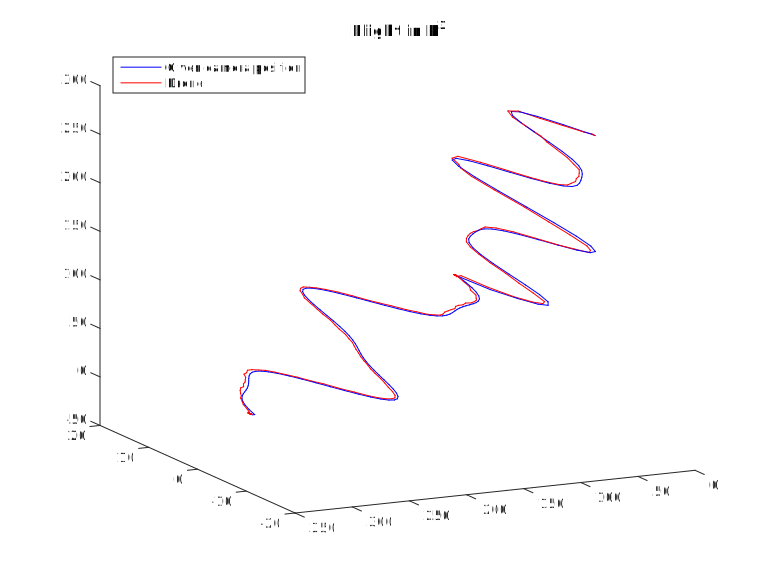
\includegraphics[width=0.9\columnwidth]{images/r3Plot.pdf}
	\end{figure}
\end{frame}

\begin{frame}
	\frametitle{Following a Skier}
	\begin{figure}
		\centering
		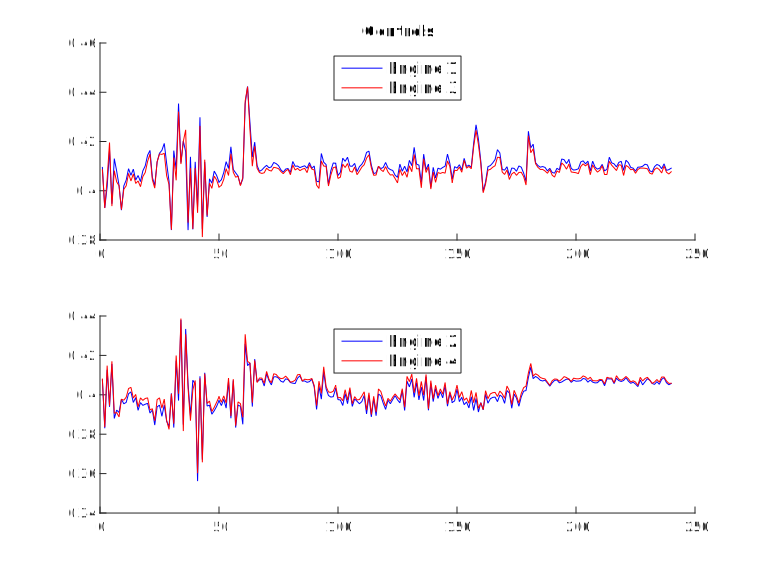
\includegraphics[width=0.9\columnwidth]{images/neu/controls.pdf}%
	\end{figure}
\end{frame}

%\begin{frame}
	%\frametitle{Following a Skier}
	%\begin{figure}
	%\centering
		%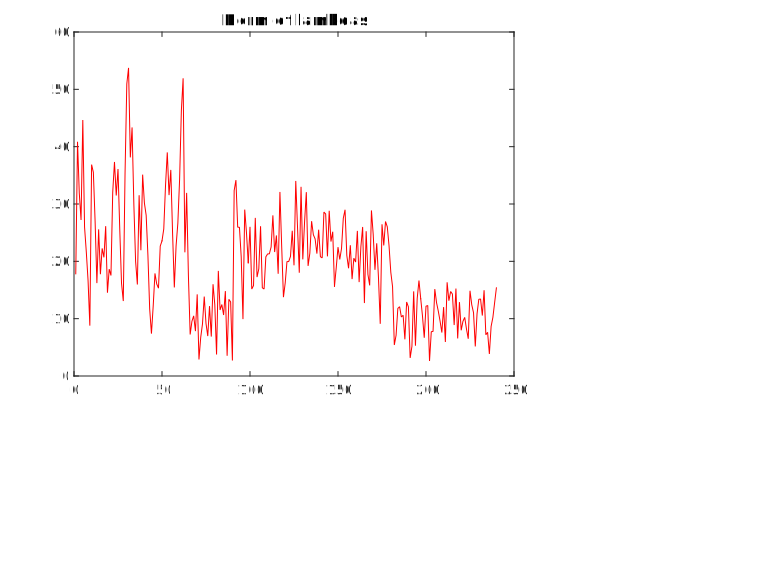
\includegraphics[width=0.85\columnwidth]{images/neu/norm_lambda.pdf}
	%\end{figure}
%\end{frame}


\nocite{Boyd2009}
\nocite{Diehl2001}
\nocite{Diehl2002}
\nocite{Diehl2005}
\nocite{Diebel2006}
\nocite{Garcia2013}
\nocite{Richter-Gebert2009}
\nocite{Reyes-Valeria2013}
\nocite{Hartmann2014}
%
\begin{frame}[allowframebreaks] % Literaturverzeichnis über mehrere Frames
 \frametitle{References}
	\bibliography{Literaturliste}
	\bibliographystyle{plain}
\end{frame}

\begin{frame}
	\frametitle{What we learned from the Project:}
	\begin{doublespace}
	\begin{itemize}
		\item you have to know your plan to ignore it
		\item MATLAB\(^{\text{\textregistered}}\) is special
		\item tests are helpful - or drive you crazy
		\item loopings can be cheap, too
		\item keep your colorscheme
		\item keep calm and do case studies
	\end{itemize}
	\end{doublespace}
\end{frame}

\begin{frame}
\frametitle{Any Questions?}
	\begin{figure}%
	
\includegraphics[width=0.9\columnwidth]{images/Easter_Egg/fairy-penguin}%
	\end{figure}
\end{frame}

\end{document}
